\section{Page de capteur}\label{sec:page-de-capteur}

    \begin{figure}[H]
        \begin{center}
            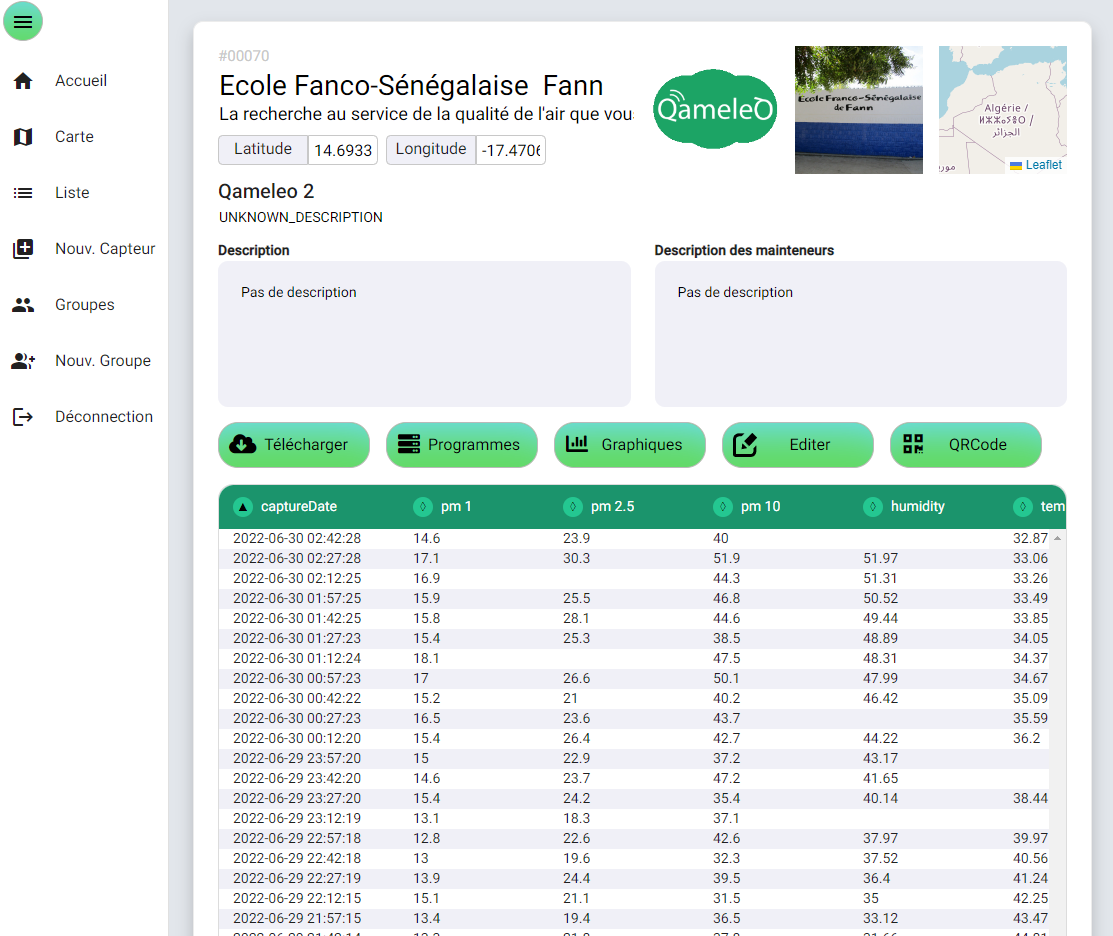
\includegraphics[width=12cm]{resources/sensor}
        \end{center}
        \caption{Page de capteur}
        \label{fig:page-de-capteur}
    \end{figure}

    Ceci est la page de présentation du capteur, elle permet de nombreuses actions :
    téléchargement des données, téléversement du programme, visualisation de graphique,
    éditions des informations du capteur et création de QRcode.
    En plus de cela elle permet d'écrire deux descriptions :
    une à destination des visiteurs et une autre pour les mainteneurs du capteur.
    Vous pouvez aussi observer les dernièrse données reçues via un tableau.